\documentclass[12pt,letterpaper]{article}           % fleqn: align equations left

% Document:
\usepackage{geometry}                                     % Custom margins for single page, etc.
\usepackage{fullpage}                                     % Use the full page
\usepackage{setspace}                                     % Enables custom margins, doublespacing, etc.
\usepackage{pdflscape}                                    % Use: \begin{landscape} ... \end{landscape}

% Font/text:
\usepackage[latin9]{inputenc}                             % Font definition and input type
\usepackage[T1]{fontenc}                                  % Font output type
\usepackage{lmodern}                                      % Latin Modern fonts
\usepackage{textcomp}   
\usepackage{multirow}                                  % Supports many additional symbols

%\usepackage[urw-garamond]{mathdesign} %dont use with amssymb, etc
%%%%Packages used without Mathdesign
\usepackage{amsmath}                                      % Math equations, etc.
\usepackage{amsthm}                                       % Math theorems, etc.
\usepackage{amsfonts}                                     % Math fonts (e.g. script fonts)
\usepackage{amssymb}                                      % Math symbols such as infinity
\DeclareMathOperator*{\Max}{Max}                          % Better looking max function
\DeclareMathOperator*{\Min}{Min}                          % Better looking min function

%%%%%%%%%%%%%%%%%%%%%%%5
\usepackage{xcolor}                                        % Enables colored text
\definecolor{darkblue}{rgb}{0.0,0.0,0.66}                 % Custom color: dark blue
\usepackage[hyperfootnotes=false,bookmarksopen]{hyperref} % Enable hyperlinks, expand menu subtree
\hypersetup{                                              % Custom hyperlink settings
    pdffitwindow=false,                                   % true: window fit to page when opened
    pdfstartview={XYZ null null 1.00},                    % Fits the default zoom of the page to 100%
    pdfnewwindow=true,                                    % Links in new window
    colorlinks=true,                                      % false: boxed links; true: colored links
    linkcolor=darkblue,                                   % Color of internal links
    citecolor=darkblue,                                   % Color of links to bibliography
    urlcolor=darkblue  }                                  % Color of external links

% Images:
\usepackage{graphicx}                                     % Allows .jpg images to be included
%\usepackage{epstopdf}                                    % Convert .eps images on the fly
%\usepackage{subfig}                                       % Enables arrayed images
\usepackage[section]{placeins}                            % Forces floats to stay in section
\usepackage{float}                                        % Used with restylefloat
\restylefloat{figure}                                     % "H" forces a figure to be "exactly here"
\usepackage[justification=centering]{caption}             % Center captions
\usepackage{subfig} %allow multiple floats in a figure



%\usepackage{datetime}                                     % Custom date format for date field
%\newdateformat{mydate}{\monthname[\THEMONTH] \THEYEAR}    % Defining month year date format
\usepackage{tikz}                                        % Timelines and other drawings
\usetikzlibrary{decorations}                             % Formating for Tikz
\usetikzlibrary{decorations.pathreplacing}
\usetikzlibrary{calc}
\usetikzlibrary{matrix}
\usetikzlibrary{positioning}
\definecolor{darkred}{rgb}{0.8,0,0}
\usepackage{tikz-3dplot}




%%%%%%%%%%%MATH
\usepackage{graphicx}
\usepackage{caption}
%\usepackage{subcaption} %this produces an error with the package subfig

%Flow Chart
\tikzstyle{decision} = [diamond, draw, fill=blue!20, text width=4.5em, text badly centered, node distance=3cm, inner sep=0pt]
\tikzstyle{block}    = [rectangle, draw, fill=black!25, text width=5em, text centered, rounded corners, minimum height=4em]
\tikzstyle{line}     = [draw, -latex']
\tikzstyle{cloud}    = [draw, ellipse,fill=red!20, node distance=3cm, minimum height=2em]

\pagestyle{empty}

%%%%%%%%%%%%%%%%%%%%%%%%%%%%%%%5
\begin{document}


\begin{center}
\begin{table}[]
\begin{tabular}{cccll}
                          & Left                     & Right                    &  &  \\ \cline{2-3}
\multicolumn{1}{c|}{Up}   & \multicolumn{1}{c|}{1,1} & \multicolumn{1}{c|}{2,0} &  &  \\ \cline{2-3}
\multicolumn{1}{c|}{Down} & \multicolumn{1}{c|}{0,2} & \multicolumn{1}{c|}{2,2} &  &  \\ \cline{2-3}
\multicolumn{1}{l}{}      & \multicolumn{1}{l}{}     & \multicolumn{1}{l}{}     &  & 
\end{tabular}
\end{table}
\end{center}

\newpage

\begin{figure}[!h]
	\centering
	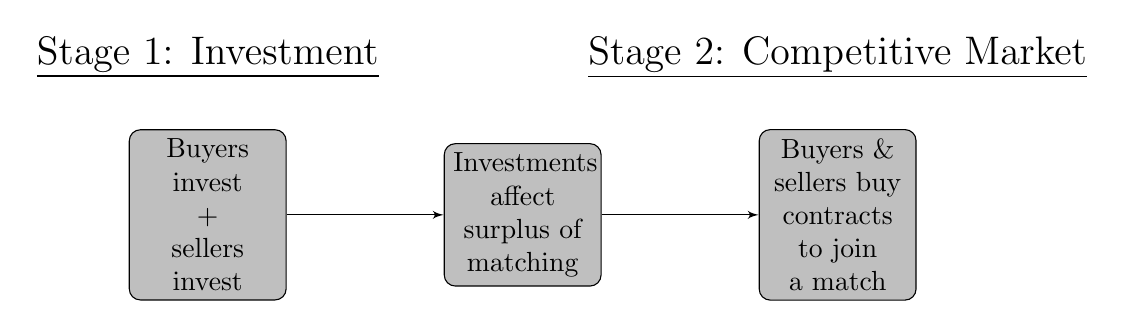
\begin{tikzpicture}[scale=0.5, node distance = 2cm, auto]
	\node [block] (st1) {Buyers invest
		\\+\\ sellers invest};
	\node [block, right of=st1, node distance=
	4cm] (st1a) {Investments affect surplus of matching};
	\node [block, right of=st1a, node distance=4cm] (st2) {Buyers \& sellers buy contracts to join a match};
	\path [line] (st1) -- (st1a);
	\path [line] (st1a) -- (st2);
	\node [above of=st1, node distance=2cm] (1) {\underline{\Large{Stage 1: Investment}}};
	\node [above of=st2, node distance=2cm] (2) {\underline{\Large{Stage 2: Competitive Market}}};
	\end{tikzpicture}
\end{figure}

\newpage

\begin{figure}[!h]
    \centering
    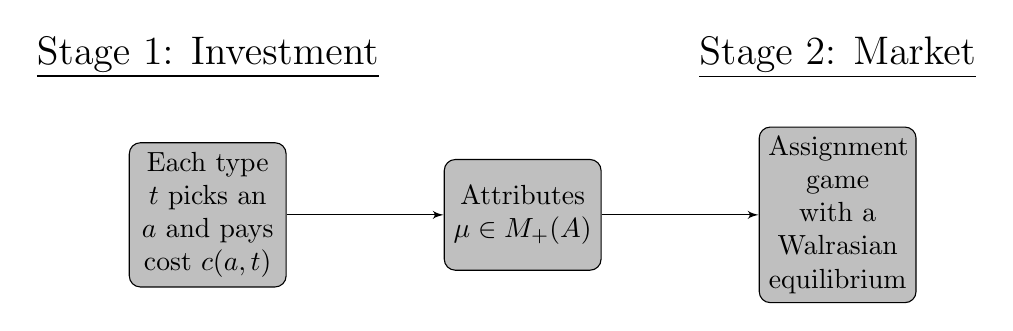
\begin{tikzpicture}[scale=0.5, node distance = 2cm, auto]
        \node [block] (st1) {Each type $t$ picks an $a$ and pays cost $c(a,t)$};
        \node [block, right of=st1, node distance=
4cm] (st1a) {Attributes $\mu \in M_+(A)$};
        \node [block, right of=st1a, node distance=4cm] (st2) {Assignment game with a Walrasian equilibrium};
        \path [line] (st1) -- (st1a);
        \path [line] (st1a) -- (st2);
		\node [above of=st1, node distance=2cm] (1) {\underline{\Large{Stage 1: Investment}}};
		\node [above of=st2, node distance=2cm] (2) {\underline{\Large{Stage 2: Market}}};
    \end{tikzpicture}
\end{figure}


\newpage

%\begin{figure}
%\begin{tikzpicture}[scale=1.5]
%\node [above] at (0.55, 1.1) {$s=1$};
%
%\node [above] at (5.3, 1.1) {$s=1$};
%
%\node [above] at (2.5, 2.2) {$b=1$};
%
%\node [above] at (2.5, 1.1) {$s=0$};
%
%\node [above] at (5.5, 2.1) {$b=0$};
%
%\node [above] at (7.5, 1.1) {$s=0$};
%
%
%\draw [fill] (1.3, 1.8) circle [radius=0.1] node [above] {Seller};
%
%\draw [fill] (6.5, 1.8) circle [radius=0.1] node [above] {Seller};
%
%\draw [fill = white] (3.9, 2.7) circle [radius=0.1] node [above] {Buyer};
%
%\draw (0, 0) node [below] {$(1/4,1/4)$}-- (1.3, 1.8) -- (3.83, 2.65);
%
%\draw (3.96, 2.65) -- (6.5, 1.8) -- (7.8, 0) node [below] {$(0,0)$};
%
%\draw (1.3, 1.8) -- (2.6, 0) node [below] {$(-1/4,0)$};
%
%\draw (6.5, 1.8) -- (5.2, 0) node [below] {$(0,-1/4)$};
%\end{tikzpicture}
%\end{figure}

\newpage


%\begin{figure}[t]
%	
%	\begin{tikzpicture}[scale=1]
%	
%	\draw [->] (0,0) node [below] {0} -- (0,0) -- (6,0) node [right] {Seller Surplus};
%	
%	\draw [->] (0,0) node [below] {0} -- (0,0) -- (0,5.5) node [above] {Buyer Surplus};
%	
%	\draw [line width=3, red](0,5)--(5,0);
%
%	\node [left] at (0,5) {$\frac{1}{2}$};
%	
%	\node [below] at (5,0) {$\frac{1}{2}$};
%	
%	\draw [fill,red] (0,0) circle [radius =0.15];
%	
%	\draw [decorate,decoration={brace,amplitude=10pt,mirror,raise=4pt},yshift=0pt]
%	(5,0) -- (0,5) node [black,midway,xshift=1cm, yshift=.75cm] {$\frac{1}{2}- p(s)$};
%	
%	\end{tikzpicture}
%	
%	
%\end{figure}
%
%\newpage

\newpage
\begin{figure}[h]
	\centering
	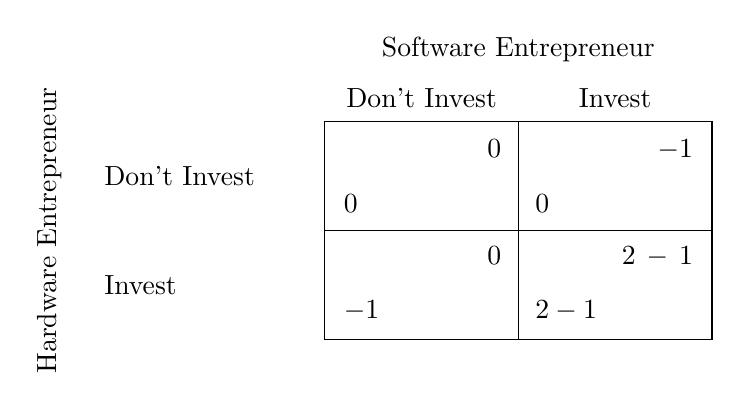
\begin{tikzpicture}
	\matrix[matrix of math nodes,every odd row/.style={align=right},every even row/.style={align=left},every node/.style={text width=2cm},row sep=0.2cm,column sep=0.2cm] (m) {
		$0$ & $- 1$\\
		$0$ & $0$\\
		$0$& $2 -1 $\\
		$- 1$&$2 - 1 $\\
	};
	\draw (m.north east) rectangle (m.south west);
	\draw (m.north) -- (m.south);
	\draw (m.east) -- (m.west);
	
	\coordinate (a) at ($(m.north west)!0.25!(m.north east)$);
	\coordinate (b) at ($(m.north west)!0.75!(m.north east)$);
	\node[above=5pt of a,anchor=base] {Don't Invest};
	\node[above=5pt of b,anchor=base] {Invest};
	
	\coordinate (c) at ($(m.north west)!0.25!(m.south west)$);
	\coordinate (d) at ($(m.north west)!0.75!(m.south west)$);
	\node[left=5pt of c,text width=2.5cm]  {Don't Invest};
	\node[left=5pt of d,text width=2.5cm]  {Invest};
	
	\node[above=18pt of m.north] (firm b) {Software Entrepreneur};
	\node[left=3.5cm of m.west,rotate=90,align=center,anchor=center] {Hardware Entrepreneur};
	
	\end{tikzpicture}\\
\end{figure}

\newpage

\begin{figure}[h]
	\centering
	\begin{tikzpicture}
	\matrix[matrix of math nodes,every odd row/.style={align=right},every even row/.style={align=left},every node/.style={text width=3.5cm},row sep=0.2cm,column sep=0.2cm] (m) {
		$ 0$ & $- \frac{1}{4}$\\
		$0$ & $0$\\
		$0 $& $\frac{1}{2}- \frac{1}{4}$\\
		$- \frac{1}{4}$&$1 - \frac{1}{2} - \frac{1}{4}$\\
	};
	\draw (m.north east) rectangle (m.south west);
	\draw (m.north) -- (m.south);
	\draw (m.east) -- (m.west);
	
	\coordinate (a) at ($(m.north west)!0.25!(m.north east)$);
	\coordinate (b) at ($(m.north west)!0.75!(m.north east)$);
	\node[above=5pt of a,anchor=base] {$s = 0$};
	\node[above=5pt of b,anchor=base] {$s=1$};
	
	\coordinate (c) at ($(m.north west)!0.25!(m.south west)$);
	\coordinate (d) at ($(m.north west)!0.75!(m.south west)$);
	\node[left=2pt of c,text width=1cm]  {$b=0$};
	\node[left=2pt of d,text width=1cm]  {$b=1$};
	
	\node[above=18pt of m.north] (firm b) {Seller};
	\node[left=1.6cm of m.west,rotate=90,align=center,anchor=center] {Buyer};
	
	\end{tikzpicture}\\
\end{figure}

\newpage

\begin{figure}[h]
	\centering
	\begin{tikzpicture}
	\matrix[matrix of math nodes,every odd row/.style={align=right},every even row/.style={align=left},every node/.style={text width=3.5cm},row sep=0.2cm,column sep=0.2cm] (m) {
		$ 0$ & $- \frac{1}{4}$\\
		$0$ & $0$\\
		$0 $& $0- \frac{1}{4}$\\
		$- \frac{1}{4}$&$1 - 1 - \frac{1}{4}$\\
	};
	\draw (m.north east) rectangle (m.south west);
	\draw (m.north) -- (m.south);
	\draw (m.east) -- (m.west);
	
	\coordinate (a) at ($(m.north west)!0.25!(m.north east)$);
	\coordinate (b) at ($(m.north west)!0.75!(m.north east)$);
	\node[above=5pt of a,anchor=base] {$s = 0$};
	\node[above=5pt of b,anchor=base] {$s=1$};
	
	\coordinate (c) at ($(m.north west)!0.25!(m.south west)$);
	\coordinate (d) at ($(m.north west)!0.75!(m.south west)$);
	\node[left=2pt of c,text width=1cm]  {$b=0$};
	\node[left=2pt of d,text width=1cm]  {$b=1$};
	
	\node[above=18pt of m.north] (firm b) {Seller};
	\node[left=1.6cm of m.west,rotate=90,align=center,anchor=center] {Buyer};
	
	\end{tikzpicture}\\
\end{figure}

\newpage


\begin{table}[]
	\begin{tabular}{lcccc}
		&                            & Buyer Payoffs         &                       & Seller Payoffs        \\ \cline{3-3} \cline{5-5} 
		& \multicolumn{1}{c|}{(0,0)} & \multicolumn{1}{c|}{$ -\tilde{p}^i(0,0)$} & \multicolumn{1}{c|}{} & \multicolumn{1}{c|}{$ \tilde{p}^j(0,0)$} \\ \cline{3-3} \cline{5-5} 
		Matching & \multicolumn{1}{c|}{(0,1)} & \multicolumn{1}{c|}{$ -\tilde{p}^i(0,1)$} & \multicolumn{1}{c|}{} & \multicolumn{1}{c|}{$ \tilde{p}^j(0,1) -\frac{1}{4}$}  \\ \cline{3-3} \cline{5-5} 
		Contract& \multicolumn{1}{c|}{(1,0)} & \multicolumn{1}{c|}{$ -\tilde{p}^i(1,0) - \frac{1}{4}$} & \multicolumn{1}{c|}{} & \multicolumn{1}{c|}{$ \tilde{p}^j(1,0)$} \\ \cline{3-3} \cline{5-5} 
		& \multicolumn{1}{c|}{(1,1)} & \multicolumn{1}{c|}{$ 1- \tilde{p}^i(1,1) - \frac{1}{4}$} & \multicolumn{1}{c|}{} & \multicolumn{1}{c|}{$ \tilde{p}^j(1,1)- \frac{1}{4}$} \\ \cline{3-3} \cline{5-5} 
	\end{tabular}
\end{table}

$ $

\newpage


\begin{table}[]
	\begin{tabular}{lcccc}
		&                            & Buyer Payoffs         &                       & Seller Payoffs        \\ \cline{3-3} \cline{5-5} 
		& \multicolumn{1}{c|}{(0,0)} & \multicolumn{1}{c|}{$ 0$} & \multicolumn{1}{c|}{} & \multicolumn{1}{c|}{$ 0$} \\ \cline{3-3} \cline{5-5} 
		Matching & \multicolumn{1}{c|}{(0,1)} & \multicolumn{1}{c|}{$0$} & \multicolumn{1}{c|}{} & \multicolumn{1}{c|}{$0 -\frac{1}{4}$}  \\ \cline{3-3} \cline{5-5} 
		Contract& \multicolumn{1}{c|}{(1,0)} & \multicolumn{1}{c|}{$ 0 - \frac{1}{4}$} & \multicolumn{1}{c|}{} & \multicolumn{1}{c|}{$ 0$} \\ \cline{3-3} \cline{5-5} 
		& \multicolumn{1}{c|}{(1,1)} & \multicolumn{1}{c|}{$ 1-p(1,1) - \frac{1}{4}$} & \multicolumn{1}{c|}{} & \multicolumn{1}{c|}{$ p(1,1)- \frac{1}{4}$} \\ \cline{3-3} \cline{5-5} 
	\end{tabular}
\end{table}

$ $

\newpage


\begin{table}[]
	\begin{tabular}{lcccc}
		&                            & Buyer Payoffs         &                       & Seller Payoffs        \\ \cline{3-3} \cline{5-5} 
		& \multicolumn{1}{c|}{(0,0)} & \multicolumn{1}{c|}{$ 0$} & \multicolumn{1}{c|}{} & \multicolumn{1}{c|}{$ 0$} \\ \cline{3-3} \cline{5-5} 
		Matching & \multicolumn{1}{c|}{(0,1)} & \multicolumn{1}{c|}{$0$} & \multicolumn{1}{c|}{} & \multicolumn{1}{c|}{$0 -\frac{1}{4}$}  \\ \cline{3-3} \cline{5-5} 
		Contract& \multicolumn{1}{c|}{(1,0)} & \multicolumn{1}{c|}{$ 0 - \frac{1}{4}$} & \multicolumn{1}{c|}{} & \multicolumn{1}{c|}{$ 0$} \\ \cline{3-3} \cline{5-5} 
		& \multicolumn{1}{c|}{\textcolor{red}{(1,1)}} & \multicolumn{1}{c|}{$ \textcolor{red}{v^i\geq0}$} & \multicolumn{1}{c|}{} & \multicolumn{1}{c|}{$\textcolor{red}{v^j\geq 0}$} \\ \cline{3-3} \cline{5-5} 
	\end{tabular}
\end{table}


$ $

\newpage


\begin{table}[]
	\begin{tabular}{lcccc}
		&                            & Buyer Payoffs         &                       & Seller Payoffs        \\ \cline{3-3} \cline{5-5} 
		& \multicolumn{1}{c|}{(0,0)} & \multicolumn{1}{c|}{$ 0$} & \multicolumn{1}{c|}{} & \multicolumn{1}{c|}{$ 0$} \\ \cline{3-3} \cline{5-5} 
		Matching & \multicolumn{1}{c|}{(0,1)} & \multicolumn{1}{c|}{$0$} & \multicolumn{1}{c|}{} & \multicolumn{1}{c|}{$0 -\frac{1}{4}$}  \\ \cline{3-3} \cline{5-5} 
		Contract& \multicolumn{1}{c|}{(1,0)} & \multicolumn{1}{c|}{$ 0 - \frac{1}{4}$} & \multicolumn{1}{c|}{} & \multicolumn{1}{c|}{$ 0$} \\ \cline{3-3} \cline{5-5} 
		& \multicolumn{1}{c|}{\textcolor{red}{(1,1)}} & \multicolumn{1}{c|}{$ 1 - \frac{1}{2}- \frac{1}{4}$} & \multicolumn{1}{c|}{} & \multicolumn{1}{c|}{$  \frac{1}{2}- \frac{1}{4}$} \\ \cline{3-3} \cline{5-5} 
	\end{tabular}
\end{table}


$ $

\newpage


\begin{table}[]
	\begin{tabular}{lcccc}
		&                            & Buyer Payoffs         &                       & Seller Payoffs        \\ \cline{3-3} \cline{5-5} 
		& \multicolumn{1}{c|}{\textcolor{red}{(0,0)}} & \multicolumn{1}{c|}{$ 0$} & \multicolumn{1}{c|}{} & \multicolumn{1}{c|}{$ 0$} \\ \cline{3-3} \cline{5-5} 
		Matching & \multicolumn{1}{c|}{(0,1)} & \multicolumn{1}{c|}{$0$} & \multicolumn{1}{c|}{} & \multicolumn{1}{c|}{$0 -\frac{1}{4}$}  \\ \cline{3-3} \cline{5-5} 
		Contract& \multicolumn{1}{c|}{(1,0)} & \multicolumn{1}{c|}{$ 0 - \frac{1}{4}$} & \multicolumn{1}{c|}{} & \multicolumn{1}{c|}{$ 0$} \\ \cline{3-3} \cline{5-5} 
		& \multicolumn{1}{c|}{(1,1)} & \multicolumn{1}{c|}{$ 1 - \textcolor{red}{1} - \frac{1}{4}$} & \multicolumn{1}{c|}{} & \multicolumn{1}{c|}{$ \textcolor{red}{0} - \frac{1}{4}$} \\ \cline{3-3} \cline{5-5} 
	\end{tabular}
\end{table}


$ $
\newpage

\begin{figure}
	
	\begin{tikzpicture}[scale=1]
	
	\node [above] at (3,6.2) {\Large Market for $(1,1)$};
	
	\draw [->] (0,0) node [below] {0} -- (0,0) -- (6,0);
	
	\node [below] at (6.4,-.1) {Quantity};
	
	\draw [->] (0,0) node [below] {0} -- (0,0) -- (0,6) node [left] {Price};
	
	
	\end{tikzpicture}
	
\end{figure}


$ $
\newpage

\begin{figure}
	
	\begin{tikzpicture}[scale=1]

	\node [above] at (3,6.2) {\Large Market for $(1,1)$};
	
	\draw [->] (0,0) node [below] {0} -- (0,0) -- (6,0);
	
	\node [below] at (6.4,-.1) {Quantity};
	
	\draw [->] (0,0) node [below] {0} -- (0,0) -- (0,6) node [left] {Price};
	
	\draw (0,5)--(4,5)--(4,0);
	
	\node [right] at (4,.5) {Buyers' Demand};
	
	\node [left] at (0,5) {$\frac{3}{4}$};
	
	\node [below] at (4,0) {$1 - \epsilon(b)$};

	\end{tikzpicture}
	
\end{figure}

$ $
\newpage

\begin{figure}
	
	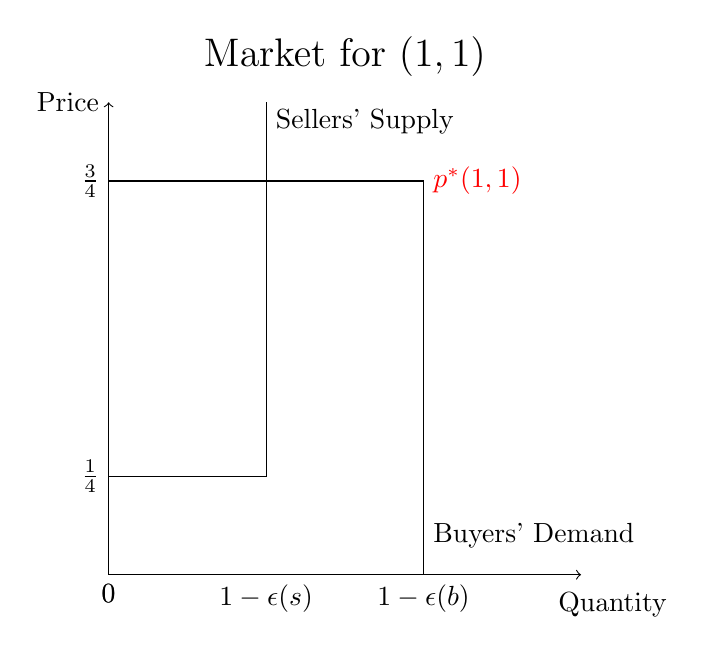
\begin{tikzpicture}[scale=1]
	
	\node [above] at (3,6.2) {\Large Market for $(1,1)$};
	
	\draw [->] (0,0) node [below] {0} -- (0,0) -- (6,0);

	\node [below] at (6.4,-.1) {Quantity};
	
	\draw [->] (0,0) node [below] {0} -- (0,0) -- (0,6) node [left] {Price};
	
	\draw (0,5)--(4,5)--(4,0);
	
	\node [right] at (4,.5) {Buyers' Demand};
	
	\node [left] at (0,5) {$\frac{3}{4}$};
	
	\node [below] at (4,0) {$1 - \epsilon(b)$};
	
	\draw (0,5/4)--(2,5/4)--(2,6);
	
	\node [right] at (2,5.75) {Sellers' Supply};
	
	\node [left] at (0,5/4) {$\frac{1}{4}$};
	
	\node [below] at (2,0) {$1 - \epsilon(s)$};
	
	\node [right,red] at (4,5) {$p^*(1,1)$};
	
	\end{tikzpicture}
	
\end{figure}

$ $
\newpage

\begin{figure}
	
	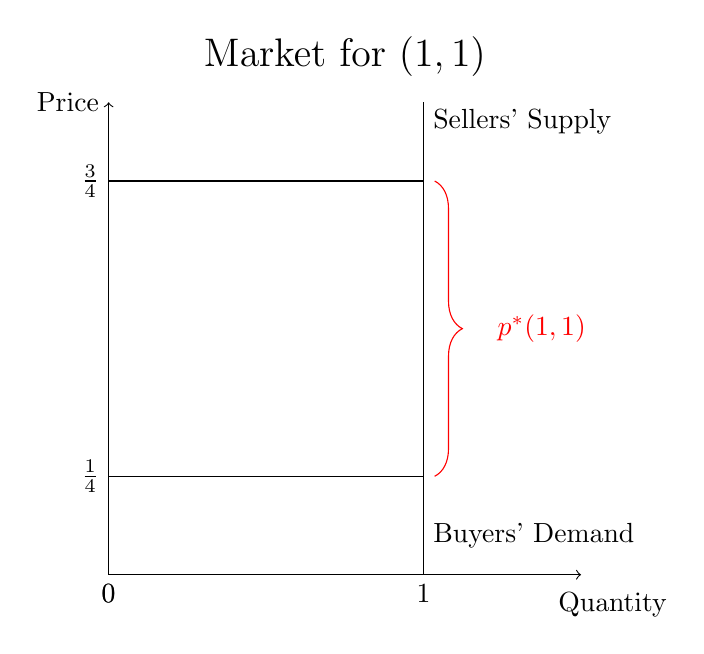
\begin{tikzpicture}[scale=1]
	
	\node [above] at (3,6.2) {\Large Market for $(1,1)$};
	
	\draw [->] (0,0) node [below] {0} -- (0,0) -- (6,0);

	\node [below] at (6.4,-.1) {Quantity};
	
	\draw [->] (0,0) node [below] {0} -- (0,0) -- (0,6) node [left] {Price};
	
	\draw (0,5)--(4,5)--(4,0);
	
	\node [right] at (4,.5) {Buyers' Demand};
	
	\node [left] at (0,5) {$\frac{3}{4}$};
	
	\node [below] at (4,0) {$1$};
	
	\draw (0,5/4)--(4,5/4)--(4,6);
	
	\node [right] at (4,5.75) {Sellers' Supply};
	
	\node [left] at (0,5/4) {$\frac{1}{4}$};
	
	\draw [red,decorate,decoration={brace,amplitude=10pt,raise=4pt},yshift=0pt]
	(4,5) -- (4,5/4) node [red,midway,xshift=1.5cm] {$p^*(1,1)$};
	
	
	\end{tikzpicture}
	
\end{figure}

\end{document}
